\chapter{Background}

\section {Website Vulnerabilities}
\label{vulnerabilities}

This project is rooted in identifying and mitigating web application vulnerabilities. In order to do so, it is essential to understand what these are, their impact, and what steps are necessary to prevent them. Fortunately, there are great wealths of information available to learn more about vulnerabilities. A great starting point is \textit{OWASP}, the Open Web Application Security Project \cite{owaspPage}. This is a community driven effort into improving the safety of software across the world, and the organisation has taken extensive steps into creating useful guides for developers wishing to know more. A particularly convenient resource they provide is a consensus of the top 10 security risks that web applications face today. \\

In their latest 2017 report, this list contains the following risks, some of which are appropriate to pursue in this project: \\

	\emph{Injection} - This risk arises from any place on a website that accepts client controlled input. There are a number of ways a website may process user input, such as the submission of web forms and search boxes, as well as using client provided URL or HTTP request parameters. Accepting this input per se is not a vulnerability, but the issue lies in blindly trusting this input to not be malicious. Whenever a server uses this input in querying a database or performing server-side commands, if the input has not been \textit{sanitized} (altered to delete potentially dangerous input combinations), there exists the risk of a leak or permanent corruption of information stored by the web application. Due to its prevalence and modus operandi, this is an appropriate vulnerability to scan for and detect in this project. \\
	
	\emph{Broken Authentication} - An application must authenticate its users so that it can confirm their identity over the internet. This is most often provided through a login form. Broken or poor authentication happens when the recommended practices to set this up are not followed. This can encompass a wide range of things, such as allowing the use of weak or default passwords, not changing default administrator account details, or poor management of session identifiers such that these can be easily manipulated. It can also include flawed password recovery mechanisms. These risks could be analysed as part of the security analysis ran by the tool, and with support from user input could be combined with scans to effectively detect weak authentication mechanisms. \\
	
	\emph{Sensitive Data Exposure} - This risk is a result of using weak cryptographic measures, or entirely foregoing their use. If a website has left their encryption keys in plaintext for someone to be able to find, or doesn't use HTTPS altogether, it may be exposed to this attack vector. The proposed tool could look for a lack of TLS enforcement across pages, and attempt a \textit{connection downgrade attack} (recognising the application does not force the use of HTTPS, and so attempting to make all requests unencrypted by using HTTP instead).  The user could make use of this information to craft an attack in attempts of finding sensitive information. \\
	
	\emph{XML External Entities} - XML (eXtensible Markup Language) is a widely used markup language to encode dcouments. The described vulnerability exists in applications that accept or include XML data from a 3rd party. A malicious user could use this data format to attempt to exfiltrate sensitive data from the handling server. Exploiting this risk without knowledgeable user input may prove to be difficult, but could be within the potential vulnerabilities considered by the tool. \\
	
	\emph{Broken Access Control} - This risk is comprised of all the possible ways in which an application might allow a user to perform actions that should be restricted to their access level (for example, a bank allowing a non-admin user to read bank balances of arbitrary accounts in the system). Determining what is and isn't an allowed action on a website varies tremendously per application, and so provides little markers for a semi-automated tool to find, and isn't ideal to try and incorporate as part of the final tool.   \\
	
	\emph{Security Misconfiguration} - A poorly setup server may suffer from this risk if there are components or services installed by default that are not prepared accordingly to the necessary security measures. An example may be disabling error stack traces from services - these may reveal information about the language being used on a database, or the version of the web server being used, which can be leveraged by an attacker in producing an exploit. This vulnerability type is well suited for automatic scans that scour the website for versioning details of services being ran, which may in turn reveal known weaknesses to look for in the case of a negligent set up.\\
	
	\emph{Cross-Site Scripting (XSS)} - One of the most well known risks for web developers today is XSS - this is exploited when a user successfully injects information into a website, causing a non-intended script to run. This is a severe risk depending on how many users it might affect. XSS may range from Self-XSS which affects only the user injecting this content, but may also be seen in the Stored-XSS variant, whereby a malicious script is stored in a database, and can be retrieved and ran by other users. This poses serious risks where credentials and other session information can be stolen. This lends itself well to the purpose of the application to be developed in this project, as it can test a wide variety of known inputs to expose this vulnerability. \\
	
	\emph{Insecure Deserialisation} - Serialisation is the process of converting a data structure into a format that can be easily transferred over a connection and understood by different programming interfaces. This resulting new format must then be deserialised to obtain the initial information back. An attacker could craft a serialized object such that it exploits the process or properties of deserialisation in the target application to obtain access to privileged data. This process will vary depending on the application domain and intended data structures, so it is not ideal for automated tools to attempt to tackle this issue.  \\ 
	
	\emph{Using components with known vulnerabilities} - In application architectures that heavily rely on a variety of components or libraries from different sources, it can often be hard to ensure that these are all kept up to date. In instances where they are not, it becomes a simple task for a scanner to produce a map of outdated version numbers to possible exploits that have been discovered on the component since then (assuming these version numbers are disclosed somewhere). Once a CVE (Common vulnerabilities and Exposures - a unique identification method for security vulnerabilities found worldwide) is published online as a result from an exploit, exploiting the web application is trivial. A scanner simply has to match the version number to a found CVE, and can reproduce exploit steps found online to endanger the application. \\ 
	
	\emph{Insufficient Logging and Monitoring} - An ideal web application keeps a track of all activities and accesses that occur. This helps provide accountability for actions. When this is not the case, it weakens the position of the website administrators to pinpoint attack culprits. This is very hard to detect from an outsider perspective, and \textit{insufficient} is an objective term; it wouldn't be fruitful to include this in an externally ran vulnerability scanner. \\
	
	In order to stay relevant, it is good not only to look at recent reports, such as the above from 2017, but also reports of different provenance. \emph{HackerOne} is a company that produces surveys harnessing the power of ethical hackers around the world to gather statistics on the current general state of web application security. In their 2017 report \cite{hackerone2017}, the survey gathers information on several vulnerability types from 2013 to 2017, and their prevalence across different industries. The most prevalent types of vulnerabilities included \textbf{Cross Site Scripting, improper authentication, Cross Site Request Forgery (CSRF), violation of secure design principles, information disclosure}  and \textbf{privilege escalation}. This should however be analysed with caution; HackerOne is a profitable company, surveying ethical hackers for hire, some of which, by self admittance, do so simply for profit or to make a living. This may therefore skew the results - it is fair to assume that some percentage of these hackers may aim for the highest ratio of bug bounty award to search / hacking efforts, so we may see more vulnerabilities discovered that are simply easier to uncover, though this may not reflect the true state of the industry. In their latest 2018 report \cite{hackerone2018}, it is clear that there are 'favourite' attack vectors by the surveyed attackers, namely, XSS and SQL injection. \\

	The aforementioned lists are not exhaustive, but are useful to consider when attempting to classify and sort different types of vulnerabilities during the development phase of this project.  There are several other features or protocols that can be checked to better ascertain the security of a website, such as:
\begin{multicols}{2}
	\begin{itemize}
	\item   Use of iFrames
	\item 	Cookies
	\item 	Appropriate headers
	\item 	Use of HTTPS
	\item   HSTS
	\item 	Javascript instrumentation
	\item 	Remote inclusion and dependency analysis
	\item 	Clickjacking
	\item 	CSP and sandboxing policies
	\end{itemize}
\end{multicols}



\section{Related Work}

This project is not the first piece of work aimed at detecting website vulnerabilities. There have been efforts in academia to address this issue (\cite{Saner, Waler, Kals:2006:SWV:1135777.1135817, stateAwareBlackBoxWebVulnScanner}, to name a few), where tools are often built as part of the related paper to demonstrate the feasibility of the proposed techniques in detecting vulnerabilities. There are also other commercial and open source tools designed to solve this problem such as \textit{Acunetix} \cite{acunetix}, IBM's \textit{AppScan} \cite{appscan} and \textit{w3af} \cite{w3af}. In order to appreciate the aspects in which this project aims to innovate in, it is fruitful to understand some aspects used to refer to these scanners.

\subsection{Black Box}

Much of the reading in this area makes reference to \textit{black box} scanners. This term is simply used for the tools that analyse a website without access to its source code. The opposite of this would be a \textit{white box} scanner - this sort of program works through static analysis on the raw code of the web application.

\begin{figure}[h]
	\centering
	\begin{subfigure}{.5\textwidth}
		\centering
		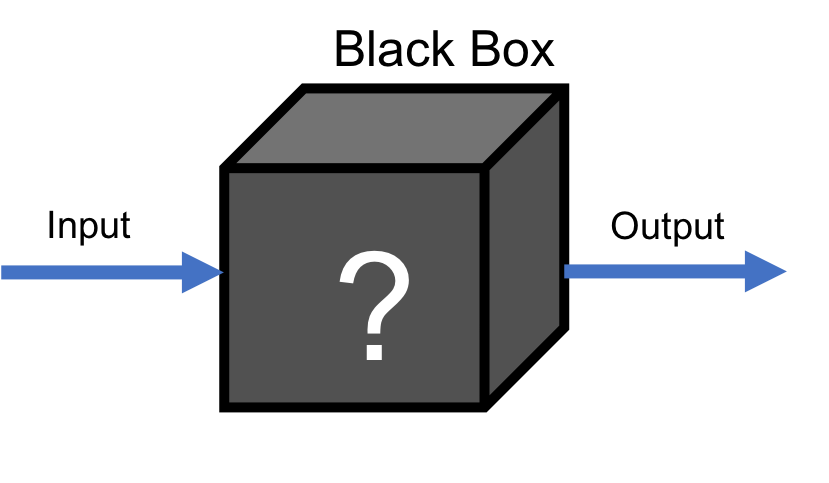
\includegraphics[width=.8\linewidth]{images/black_box.png}
		\label{fig:blackBox}
	\end{subfigure}%
	\begin{subfigure}{.5\textwidth}
		\centering
		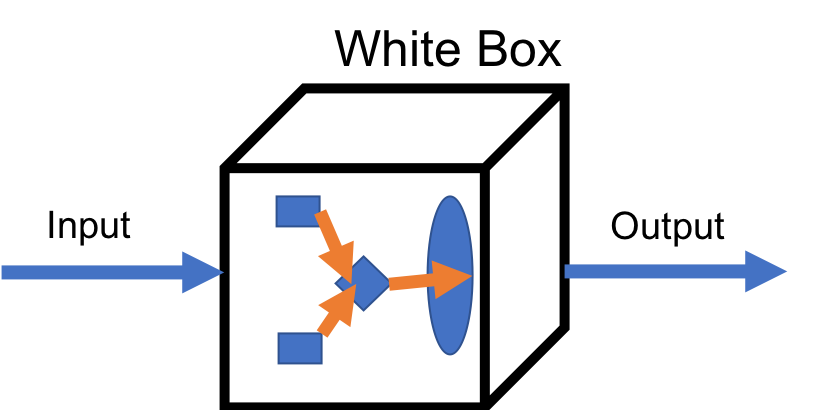
\includegraphics[width=.8\linewidth]{images/white_box.png}
		\label{fig:whiteBox}
	\end{subfigure}
	\caption{A black box scanner derives behaviour strictly from I/O, whilst a white box scanner has all the inner workings of a (web) application at its disposal for analysis}
	\label{fig:test}
\end{figure}


 A white box scanner takes into consideration the implementation of the service, so it may be designed with the specific framework or language used for the application in mind. Conversely, a black box implementation does not care about these details and looks only at outputs from the service. A major differentiation between the two approaches is their use case; a white box scanner emulates the experience of a web developer who is looking to detect potentially exposed parts of his code, whereas a black box scanner portrays the setting for a malicious attacker, where they are only working with the exterior interface of the application to forge an intrusion. The black box approach is the one I will be using in the extension implementation as it aligns best with the project requisites.

\subsection{Automated Vulnerability Scanners}
 
A large majority of web vulnerability scanners are designed to be ran passively. This means an auditor of the security of a web application would start the tool, and depending on the length and intensity of the scan, either grab a coffee while it executes or leave it running overnight. Either way, these are expected to produce reports on where a website is suffering from a vulnerability, which can then be interpreted to produce a fix. This automation is a great bonus because it makes life easier for the auditor, as they can get on with other tasks in the meantime; depending on the initial monetary and time investment needed to set up the scan, doing so automatically can be a cost-effective solution for many businesses. \\

There have been studies committed to evaluate the effectiveness of these black box scanners. Doup\'e, Cova and Vigna did an extensive analysis of the tools available in 2010 \cite{whyJohnnyCantPentest}, including tools ranging from free to \$30,000+ worth. In the same year, Bau, Bursztein, Gupta and Mitchell published their own paper with a similar analysis \cite{stateOfArtAutomatedBlackBoxWebAppVulnTesting}. More recently, in 2015, Parvez, Zavarsky and Khoury released a study on the effectiveness of scanners in detecting a limited set of vulnerabilities \cite{analysisOfEffectivenessOfBlackBoxWebAppScannersStoredSQLStoredXSS}. \\

Doup\'e et al. found that \textit{crawling} was one of the major limiting factors of web vulnerability scanners; according to them, {"...crawling is arguably the most important part of a web application vulnerability scanner; if the scanner’s attack engine is poor, it might miss a vulnerability, but if its crawling engine is poor and cannot reach the vulnerability, then it will surely miss the vulnerability"}. To better understand this, it is important to contextualise what \textit{crawling} is. \\

A typical vulnerability scanner will loosely consist of 3 different modules:

\begin{itemize}
	
	\item \textit{Crawling module} - This is the first part of the scanner that gets executed. A crawler will recursively follow every possible link in a webpage so that the tool can build up an internal representation / database of what the target website looks like. As mentioned above, this stage will make or break the scan - though it is unlikely that a crawler will be able to find 100\% of the available subpages on the target website, any missed links will result in the scanner not considering those pages, which in the worst case scenario may miss a page which is the root of many vulnerabilities on the target site. Acunetix themselves, the providers of the commercial vulnerability scanner, say "if you can't crawl it, you can't scan it!" \cite{acunetixQuoteCrawling}. 
	
	\item \textit{Attacker module} - At this stage, the scanner attempts to chip away at any potential cracks in the website. It goes through every stored entry in the previous phase and scans the content of the associated page. Depending on this content (e.g. a form or a URL parameter), the scanner issues web requests with specially crafted input designed to create \textit{interesting} responses from the web server.
	
	\item \textit{Analysis module} - This module reads the outputs from the target to the attacker module input, and scans for any significant or telling change from the server side response. If the web server generates a wildly different response to a normal input (e.g. it issues a page containing an SQL error message), then this is flagged up as a potential vulnerability. This module can have a feedback loop to the attacker module to refine attack methods. This is done through \textit{fuzzing} - creating mutations of the benign input and testing these on the application until a more malicious input is generated that triggers a vulnerability. The scan completes after all potential mutations and attack vectors have been exhausted, or a resource cap is met (time elapsed, bytes sent etc).
\end{itemize}


\begin{figure}[h]
	\centering
	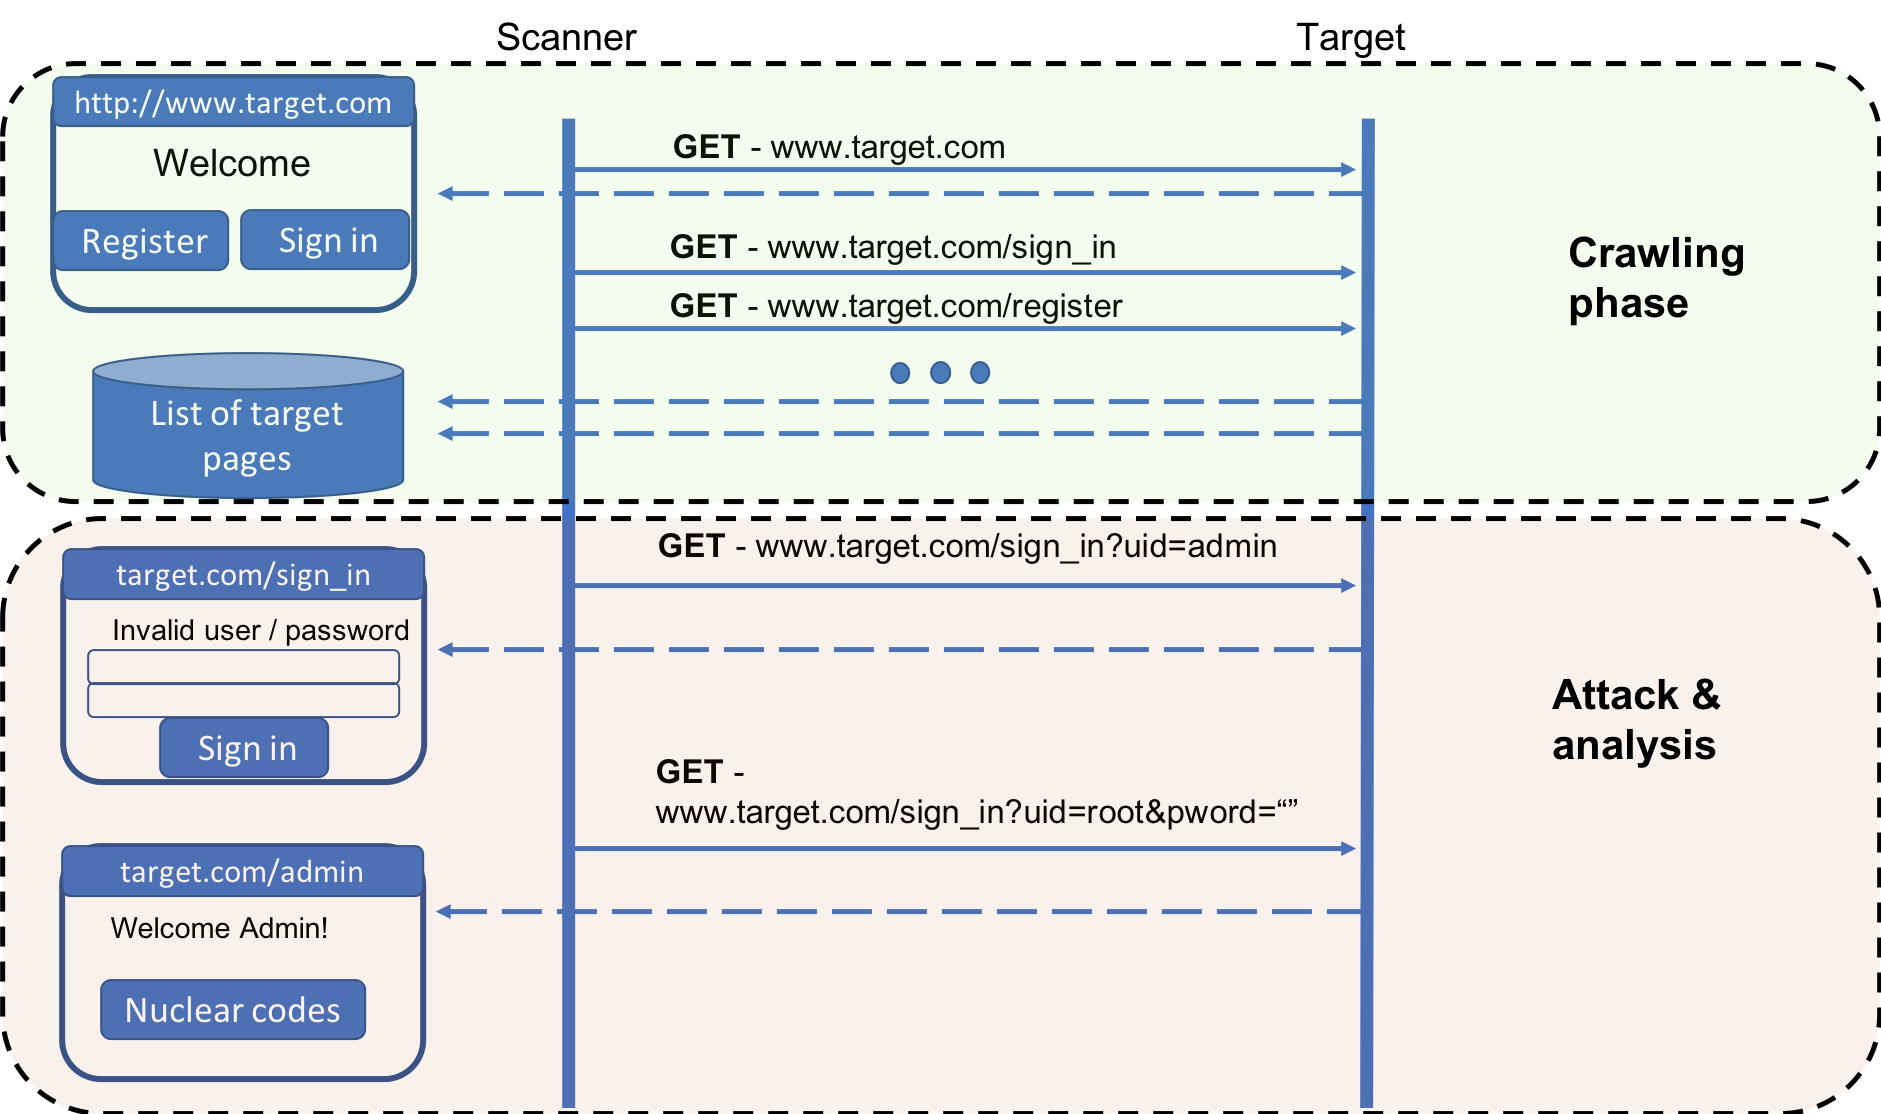
\includegraphics[width=\textwidth]{images/scanner_structure.png}
	\caption{The typical structure of a vulnerability scanner. The crawling phase builds up a database of potential pages to attack. During attack, malicious inputs are fired towards pages to try and trigger undesired behaviour - the analyser reads response contents with some heuristics to determine what responses seem to indicate vulnerabilities.}
	\label{fig:test}
\end{figure}

With this knowledge in mind, it is now easier to appreciate how important the crawling phase is, as it sets an upper bound to how far a scanner can go. Crawling in itself is however not a trivial task to implement. A naive approach to this would be to start at the target page given, scan for any \texttt{<a>} anchor links in this page and filter this list to only include links that belong to the target domain (e.g. if our target was \texttt{facebook.com}, we might be interested in \texttt{facebook.com/account}, but we would discard any links to \texttt{google.com}, as Google links belong to a different domain. As a general rule of thumb, the links we explore have the target link as a prefix to the URL). This method of crawling pages would quickly come up against issues though. A lot of the interesting state of a web application is often hidden behind a login form, so if a valid user account isn't created then a scanner will not be able to explore the full array of actions available. The method described above would not consider this, so would skip out on all the intriguing parts of a website that requires you to have an account. There are also other technologies used in the web that make this slightly harder, such as Flash objects that contain useful sublinks. These objects are not straightforward to analyse, and make automated crawling difficult. \\

This combination of components quickly complicates things for creation of an effective crawler implementation. A competent crawler needs to go above and beyond being just a database of pages - it has to emulate human interactions with an application without any prior domain knowledge. To do so, it has to somehow derive an internal representation of what the website looks like, and refer to this state when crawling and in the analysis phase. Keeping state was an issue raised by Doup\'e et al. in \cite{whyJohnnyCantPentest}. As an example of its importance, if during the attacking phase the scanner is logged in, and an attack request causes the scanner to log out of the application, all the subsequent requests will execute in a different context where the scanner is logged out, invalidating their intended purpose. Doup\'e, Cavedon, Kruegel and Vigna later addressed this by creating a scanner that generated an internal state machine representation of a web application based on heuristically unique server responses \cite{stateAwareBlackBoxWebVulnScanner}. The techniques demonstrated in that paper were useful in creating a more effective crawler that remembered state so as to not waste computation efforts. The resulting scanner achieved higher code coverage rates for web applications analysed over other otherwise similar, open-source scanners. Higher code coverage rates mean that a scanner is exercising more of the application's source code, thus increasing likelihoods of finding a vulnerability. \\

It is clear that an automated crawler based web vulnerability scanner is a difficult tool to create. The shotgun approach used by the crawler can also have negative consequences for the application as discussed in \ref{ethics}. Though state of the art crawlers can now handle the aforementioned hurdles and other intricacies of different web applications, the creation of an efficient, fully automated crawler could warrant a project of its own. \\

 
\section{Browser extensions}

I propose to create the tool described as a browser extension in Google Chrome. An extension seems to be ideal as a method to accomplish the intended functionality for 2 main reasons.

\begin{itemize}
	\item \emph{Extension privileges} - A browser extension works as a self-contained application that is trusted enough to expand the browser experience. Chrome predefines a potential permission set an extension can tap into. Each extension must declare which of these it will be using in a \texttt{manifest.json} file, as well as list of which domains it expects to be ran on. Upon installing the extension, the user is asked whether they wish to allow this behaviour. As required by the project, an extension can contact remote servers (allowing it to replay user actions on their behalf), as long as the appropriate cross origin permissions are appropriately set up.
	If an extension is compromised, the application of the least privilege principle can mitigate potential damages because it will only be able to possibly affect the declared domains at the previously granted permission level. It is therefore good practice to declare the minimum amount of domains and permissions required to get the extension to work. 
	
	An extension has a \texttt{background.html}, a page which runs invisibly as the user browses. This is where most of the logic and state of the extension is stored, but it cannot directly interact with target pages. For this, there are \textit{content scripts}; these are small Javascript programs that are injected into the selected domains and can interact with the Document Object Model (DOM) of a website and modify it according to the programmed needs. It is important for extension behaviour to not break functionality of existing sites. For example, if a web application is using JQuery 1.0 and the extension is using JQuery 2.0, it would be unacceptable for the newer dependency on the library to break the existing functionality, so content scripts are isolated from the existing page scripts. This is done through \emph{isolated worlds}, which create a sandboxed copy of the website DOM to avoid clashing between content and scripts and existing scripts. Because the content script can interact only with the website, it may be desirable to establish communication with the extension core to send information back to the \texttt{background.html} to process. For this reason, there exists a message listening API between the \texttt{background.html} and the content script to allow communication. 
	
	It is important to keep these separate for security reasons. If a content script is compromised by a malicious page targeting the extension, the attacker still has to exploit another vulnerability in the background page to exfiltrate any data. Additionally, the entire extension itself runs in a separate process to the browser and other extensions. This means if an extension is compromised and begins to degrade the system, this process can simply be halted without killing the browser or other innocent extensions.
	
	Additionally, extensions run on HTML5, CSS3 and support Javascript running on Chrome's own engine, with native JSON capabilities. They support the latest web technologies and as such are not heavily restricted on the use of these, as other methods used in black box scanners are. Therefore, browser extensions run at the appropriate level of abstraction to perform the necessary technical operations without much hinderance. 
	
	\begin{figure}[h]
		\centering
		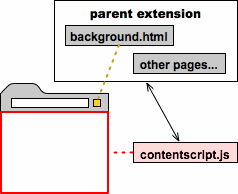
\includegraphics[width=0.4\textwidth]{images/extension_arch.png}
		\caption{An extension is split into 2 main areas. The \texttt{background.html} page has access to all extension privileges and is where the business logic of the extension is stored. It cannot interact with user webpages. Content scripts can be injected to interact with the DOM of a page. The \texttt{background.html} can contact the content script via a message passing API. Image courtesy of Google Developer documentation. \cite{chromeExtensionArchitecture}}
		\label{fig:test}
	\end{figure}
	
	\item \emph{User operability} - Because of the features described above, the extension can be designed in such a way that allows it to sit between the user and the web application and seamlessly create the desired semi-automated experience. Wherever possible, depending on the type of vulnerability, it would be ideal to give the user interactive visual cues for when the scan has detected something that merits further research. If the vulnerability is attached to a specific form that takes user input for example, the extension should have the capabilities of identifying the DOM object for this, and add a small tooltip around the visual area of this object to initiate the deeper scan analysis. If the vulnerability is not necessarily caused by visible means, then the extension is also able to create other appropriate visual cues, such as a fixed position element. 
	Being able to implement these characteristics should result in a more intuitive user experience. 
	
	This also means that the user will not be doing any heavy lifting - the extension will be passively searching for vulnerabilities as they use the website, but should also be able to be activated at user will. During the phase where the tool begins to replicate user actions to investigate a vulnerability (explained further in \ref{contribution}), if implemented appropriately, the extension will be able to repeat the human steps of submission and navigation at a much faster rate than a human would do, with several more inputs.
	
\end{itemize} 


\section{Project Contribution}
\label{contribution}

These points lead us nicely onto the intended innovation behind the project idea - to create a semi-automated web application vulnerability scanner. The essential difference between this and the aforementioned black box scanners is that it intends to work as an aide alongside a pentester, not as a fully automated background process. \\

The proposition of creating a tool that is driven by user input seems appealing for a number of reasons:

\begin{itemize}
	\item \textbf{Full Experience} - A scanner that analyses a web application for vulnerabilities as a user is using the application has fewer limitations as to what is within its scope. As pointed out by \cite{whyJohnnyCantPentest}, scanners struggle to scour through more complex constructs of the internet such as convoluted Javascript forms, AJAX requests and Flash objects. As a result, many scanners ignore these features altogether, dismissing potential vulnerabilities in the process. A user driven experience allows the user to interact as they would normally with these technologies, and can analyse inputs and outputs accordingly.
	
	\item \textbf{Educational} - As mentioned above, one of the issues that leads to the need of vulnerability scanners is the lack of security-aware developers. By developing a tool that works alongside developers, they can refine their skills in this area if they already know some security basics. There is also room for learning for website owners as penetration testers may demonstrate the severity of exploits caused by vulnerabilities using the tool, and mitigating these. 
	
	\item \textbf{Simpler crawling module} - Since the tool is not scouring the entire site at once but is rather following the more natural workflow of a human user, the equivalent crawling module will only need to keep a much smaller representation of the website as opposed to before. A proposed methodology to simplify this process given the project specification is to create a crawler based on recommendations and an 'action replay' mechanism. 
	
	The recommendation algorithm will need to be based off of similar existing algorithms in automatic crawlers. Since the tool must be driven by user input, the crawler would analyse contents and interactions of the web application with the user (as it would do automatically), and suggest specific features to the user as a starting point for the scan. This can be done by passively reading the contents of web requests between the user and the web application and flagging up any that seem to exhibit behaviour of an insecure system, such as passing user inputs in clear text, or using client-side inputs to control important application sensitive logic. Once a user chooses to follow a recommendation, they may investigate the flagged feature more closely.
	
	At this point, the 'action replay' algorithm begins - once a user has elected a potential target to test for a vulnerability, the tool begins to record user actions. Depending on the selected feature and what vulnerabilities may be discoverable, the tool can then suggest a stopping point of recording, or wait for the user to determine when their actions that detect a vulnerability are enough. The tool then takes these actions and analyses their outputs - it may be the case that a user has found a vulnerability on their first go. It could also be the case that this input didn't trigger a vulnerability, but is worth looking into further. At this point, the crawler will begin to fuzz different versions of input that may be more effective at showcasing vulnerabilities. In recent research by Parvez et al. into evaluating black box scanners \cite{analysisOfEffectivenessOfBlackBoxWebAppScannersStoredSQLStoredXSS}, one of the final recommendations for a better scanner was to add interactive multistep options to the scanner, which is a main focus of this method. To the best of my knowledge, this 'action replay' algorithm is a novel approach in this area.
	
	\begin{figure}[h]
		\centering
		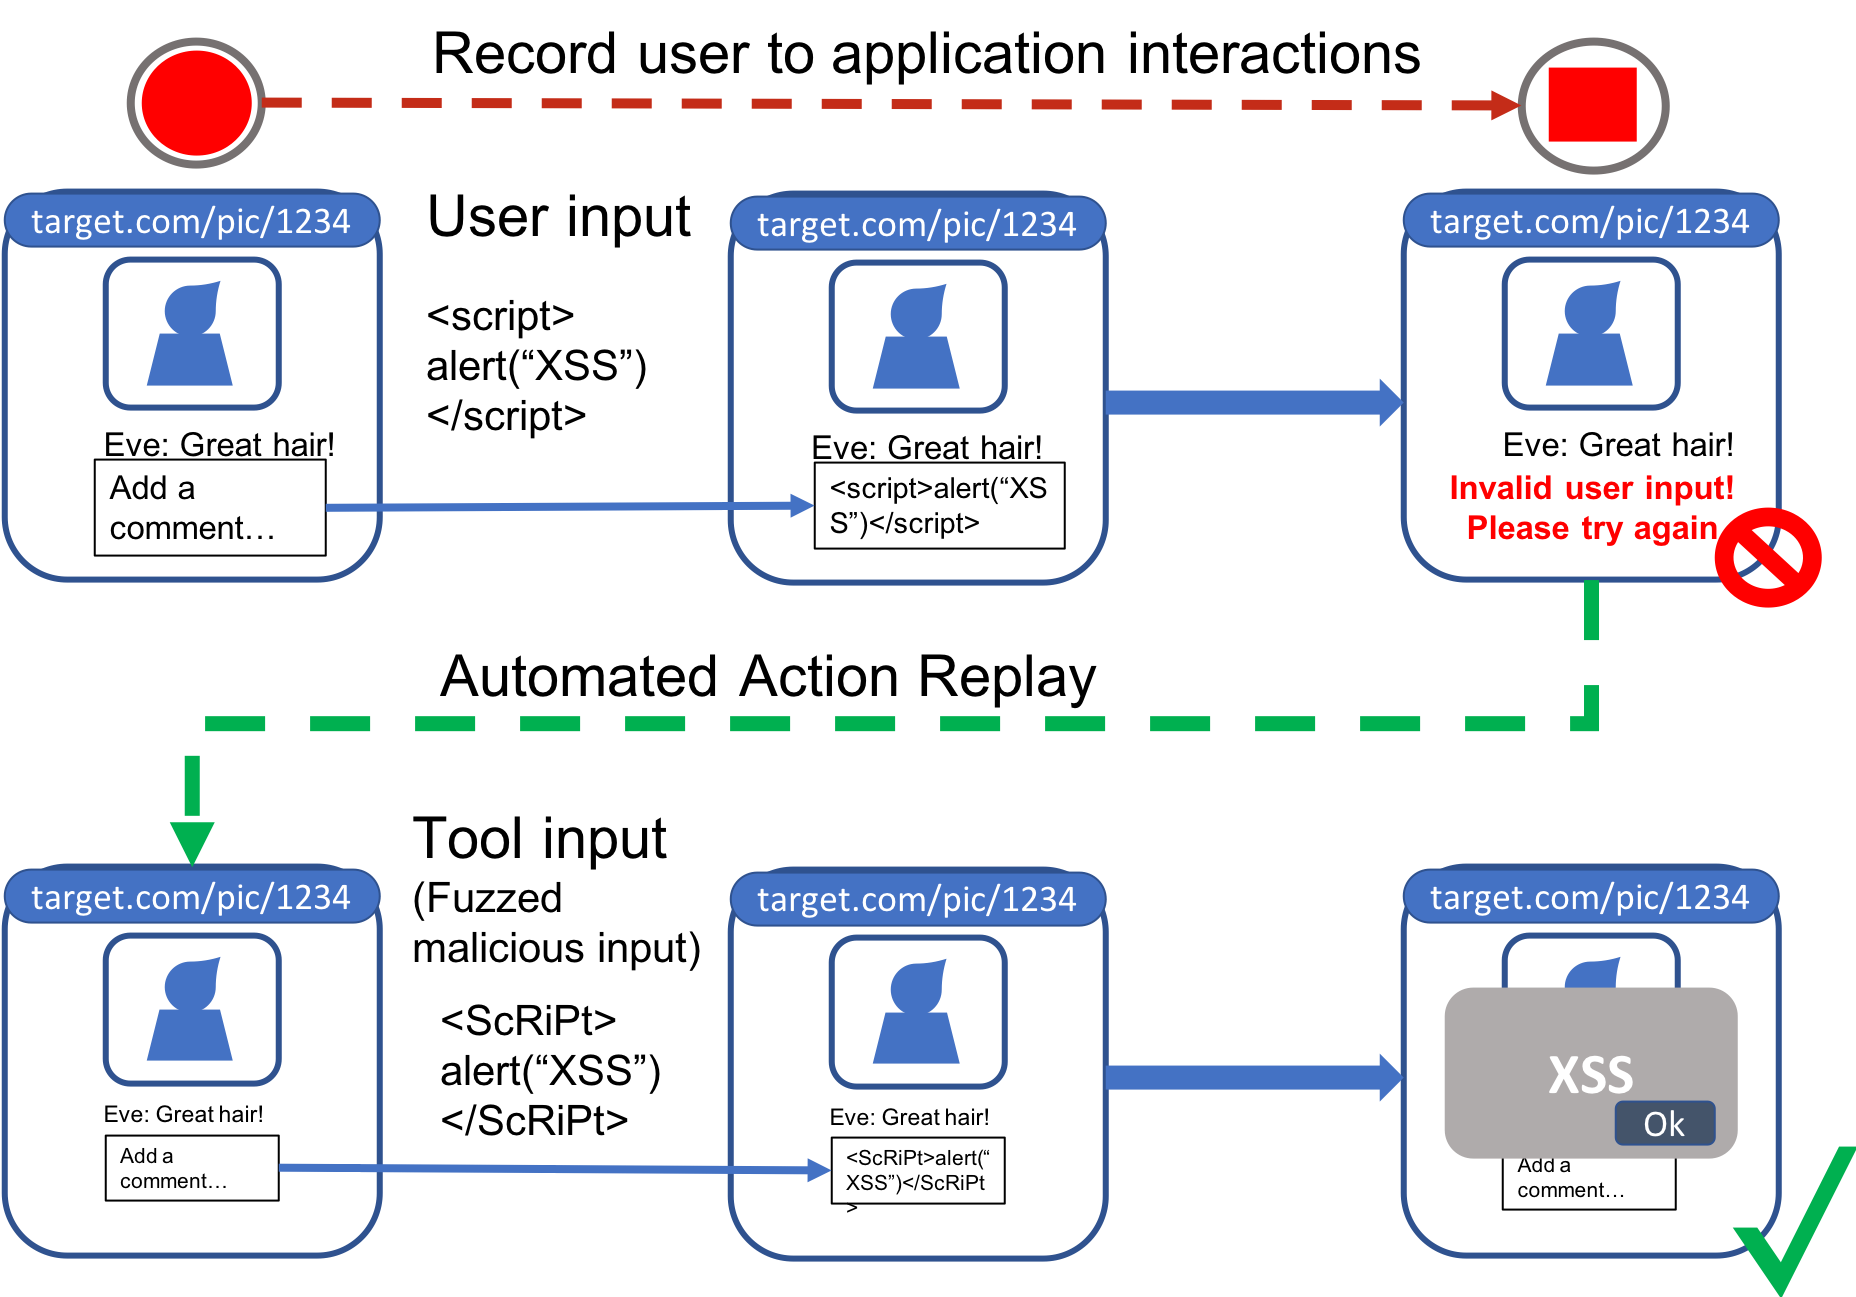
\includegraphics[width=\textwidth]{images/action_replay.png}
		\caption{A visualization of the proposed action replay algorithm. The tool records user input for a time period determined by the user. The tool then replicates actions using fuzzed inputs to try and uncover vulnerabilities if the first attempt was unsuccessful.}
		\label{fig:test}
	\end{figure}
	
	
	\item \textbf{Human judgement} - The previously mentioned paper by Parvez et al. also mentions that choosing the right attack vectors to exploit vulnerabilities is still a big challenge for black box scanners \cite{analysisOfEffectivenessOfBlackBoxWebAppScannersStoredSQLStoredXSS}. Huang et al. recently built a scanner that performed well against open-source competition \cite{webAppSecThreatsCountermeasuresPitfalls}. However, these authors recently acknowledge that \emph{"there is no silver bullet for web application security; threats will continue to grow and evolve"}. Herein lies much of the motivation for making this project user-centric: vulnerability detection and even exploitation may be automated \cite{darpaAIChallenge}, but for now, efforts in having to build an AI that is able to do this are astronomical - it takes years for teams of experts to build tools that do this. Following its recent success, the winner of the DARPA Cyber Grand Challenge (an AI-only capture the flag contest) was pitted against human professionals at the 2016 DEF CON CTF Challenge, where it came last \cite{defcon16Results}. These efforts show a bright future for fully automated security systems, but these may still be some years away in the full making. This project does not admit defeat in attempting to automate the process of countering malicious agents, but rather aims to increase the likelihood of doing a good job against them by covering our bases with higher quality base defences. In fact, even limited domain knowledge has shown to be useful for human penetration testers; a group of students with 'average' security skills achieved a higher success rate on their own than some vulnerability scanners in analysing web applications \cite{whyJohnnyCantPentest}. It is hoped that with the correct suggestions provided by the tool, this project lowers the minimum requirements of a successful user to be 'below average' in their security domain knowledge. \\

\end{itemize}


 
\section{Limitations}
\label{limitations}

In order to be able to effectively evaluate this project at a later point, it is important to delineate realistic expectations in terms of what it can and cannot do. 

\subsection{Time taken}
Since the extension is user driven and not fully automatic, the suggested process will be inevitably slower than if it was otherwise automated - there will be waiting times as users will not instantly attempt to uncover recommended vulnerabilities. There may also be some intellectual effort involved in crafting initial input to try and do this, which adds to this. Both of these factors add to 2 different metrics: the total scan time and the time taken from recommendation to decision of whether a vulnerability is found or not. \\

Total scan time may be especially hard to measure, and can be seen as a disadvantage of this scan. It is not known whether a user will eventually go through every possible page that is relevant, so it becomes very difficult to claim an end to the scan. On the contrary, automated crawlers \emph{will eventually} come to an end their search, and thus put an upper bound on how many resources they can analyse. Human driven crawling may stop or resume at any given point. Not being able to best assess the total scan time is an acceptable tradeoff of this project as it will simply not be avoidable given human driven interaction is being explored. \\

The time taken to ascertain whether a vulnerability exists or not from a recommendation can however be bounded. This period begins when a user decides to investigate a recommendation on their own or by suggestion of the tool, and finishes either when enough proof of a vulnerability has been observed, or when all possible fuzzing opportunities in exploiting it have been exhausted - the extension will have a list of possible fuzzing mutations per type of vulnerability, so this work is bounded by that list. Again, since this is not a fully automated tool, the extension is expected to take longer in this metric due to human interaction when comparing it to automated scanners, which is only natural. \\

 \subsection{Breadth of  work}
 Section \ref{vulnerabilities} describes many potential kinds of vulnerabilities that the project may choose to tackle. Some of these are harder to detect than others, and thus require more development work. This large scope may make it tempting to try and undertake too many things at once. At the time of writing, it is also hard to assess just how difficult it may be to implement scanning for a specific type of vulnerability. The extension will be developed with aims of finding revelant vulnerabilities - sorted by both volume of occurrence and contemporary relevance as found on surveys. One of the most recurring vulnerabilities in both aspects is Cross Site Scripting, so developing the tool to be able to detect this class of weaknesses is a good starting point. Other features that may seem small (such as analysing cookies or the use of iFrames on a page), may also be beneficial to implement. As the project develops, it becomes harder to weigh the costs of effort to implement versus the success rate of focusing on a specific feature, so some further time should be allocated to allow for this meta research. \\ 
 
 \subsection{Self security}
 	The security of the extension being developed should not be taken for granted. As mentioned above, Google Chrome has several mechanisms in place to safeguard extensions from falling prey to malicious attackers. Namely, these are:
 	\begin{itemize}
 		\item \textit{Isolated Worlds}
 		\item Privilege separation
 		\item Predefined permissions
 		\item CSP (Content Security Policy)
 	\end{itemize} 
 	Although these practices make it much easier for a developer to avoid serious mistakes, it is still possible to write vulnerable extensions. The \textit{threat model} in this case (the way we choose to archetype our potential enemy), is by means of a web attacker. This would be someone who sets up a 'honeypot' website, expecting the extension to scan it but in the process attempt to compromise the extension by different means. Due to the priveleges granted to an extension, this may result in the jeopardizing of sensitive user data, such as their passwords. A recent paper by Carlini, Felt and Wagner reinforces the notion that Chrome's existing techniques are effective in preventing extension compromise, but also list some developer practices that could result in vulnerabilities, such as the unrestricted use of the \texttt{eval} function by Javascript (which is known to be dangerous as it executes given strings as commands), and injecting website data into HTML \cite{evalChromeExtensionSecurityArchitecture}. Many of the notions mentioned in the paper are also cited in Google's own documentation on how to write Chrome extensions \cite{chromeExtensionArchitecture}. Following these best practices will decrease potential risks associated with this project. \\ 

\subsection{Ethics \& Handling of Results}
\label{ethics}
This project aims to build a tool that helps users find vulnerabilities in web applications. Obviously, this may raise ethical ramifications as to how the tool interacts with websites, and how its output is handled. \\

As the tool needs to send requests on the user behalf when executing (especially so during the 'action replay' phase described above), the rate at which this is done may be of concern. Conventional automated scanners may fire 100's of different fuzz attempts at a web application, \emph{per vulnerability, per existing page} - a shotgun-like approach. This approach is very intensive, and for web applications set up for smaller amounts of traffic, may result in a Denial of Service (DoS). This tool aims to reduce this by only passively reading user crawled content, and only actively interacting with the website whenever a flagged vulnerability has been detected. \\

A related concern is to do with the scope of testing and uses on a real web application. For testing and evaluation purposes, the tool will be ran against existing, known to be vulnerable applications, such as DVWA \cite{dvwaSite}. Ideally, it should also be ran against other web applications beyond my control. However, for some of these, it may be the case that running the unhinged extension may infringe usage terms and agreements. For this purpose, a proposed restrained mode for the tool may be built, such that it does not actively take any action when browsing web applications, but rather only passively reads network traffic to deduce and recommend potential vulnerabilities. \\

Naturally, as per the project ideals, any vulnerabilities that may be found as a result of running this extension will duly be reported to the appropriate developers.